
%(BEGIN_QUESTION)
% Copyright 2006, Tony R. Kuphaldt, released under the Creative Commons Attribution License (v 1.0)
% This means you may do almost anything with this work of mine, so long as you give me proper credit

Suppose a constant flow rate of 20 gallons per minute enters the vessel through the pipe.  Graph this constant value of flow over time, as well as the accumulating volume of liquid inside the vessel over time:

$$\includegraphics[width=15.5cm]{i01579x01.eps}$$

Assume the vessel is completely empty when the liquid begins to flow at start time (0:00).  Note that the unit of time for the graph's horizontal axis is minutes:seconds, not hours:minutes.  Also, explain why the assumption of an empty vessel at 0:00 is important for predicting total stored volume in the vessel.

\filbreak

Calculate the accumulated liquid volume at the following times:

\medskip 
\item{}Time = 1:00; Volume = \underbar{\hskip 50pt}
\vskip 5pt
\item{}Time = 1:30; Volume = \underbar{\hskip 50pt}
\vskip 5pt
\item{}Time = 2:00; Volume = \underbar{\hskip 50pt}
\vskip 5pt
\item{}Time = 2:30; Volume = \underbar{\hskip 50pt}
\vskip 5pt
\item{}Time = 2:45; Volume = \underbar{\hskip 50pt}
\end{itemize} 

\underbar{file i01579}
%(END_QUESTION)





%(BEGIN_ANSWER)

$$\includegraphics[width=15.5cm]{i01579x02.eps}$$

I will let you explain the importance of assuming an empty vessel to start!

\medskip 
\item{}Time = 1:00; Volume = 20 gallons
\item{}Time = 1:30; Volume = 30 gallons
\item{}Time = 2:00; Volume = 40 gallons
\item{}Time = 2:30; Volume = 50 gallons
\item{}Time = 2:45; Volume = 55 gallons
\end{itemize} 

%(END_ANSWER)





%(BEGIN_NOTES)

The importance of assuming an empty vessel to start is that integration only tells us how much the volume will increase past its starting value at 0:00, not how much liquid is held by the vessel, absolute!  What we are looking at here is the so-called {\it constant of integration} problem.  The integration formula for this scenario needs to have an ``initial volume'' constant $V_0$ added to the integral in order to be complete:

$$V = \int Q \> dt + V_0$$

%INDEX% Mathematics, calculus: integral (accumulated volume as the integral of flow)

%(END_NOTES)


